\documentclass[11pt,a4paper]{article}
\usepackage{fontspec}
\setmainfont{TeX Gyre Pagella}
\newfontfamily\headfont{Inter}[UprightFont=*-ExtraBold,BoldFont=*-ExtraBold,Extension=.otf,Path=/usr/share/fonts/opentype/inter/]
\usepackage[a4paper,margin=2.3cm]{geometry}
\usepackage{graphicx,booktabs,float,caption,array,xcolor,longtable}
\usepackage{xurl}
\usepackage[hidelinks]{hyperref}
\usepackage{titlesec}
\usepackage[round]{natbib}
\usepackage{setspace}
\setstretch{1.05}
\renewcommand{\topfraction}{0.9}
\renewcommand{\bottomfraction}{0.8}
\renewcommand{\textfraction}{0.1}
\renewcommand{\floatpagefraction}{0.75}
\setlength{\parindent}{0pt}
\setlength{\parskip}{0.55em}
\titleformat{\section}{\headfont\Large}{\thesection}{0.8em}{}
\titleformat{\subsection}{\headfont\large}{\thesubsection}{0.8em}{}
\captionsetup{font=small,labelfont=bf}
\urlstyle{same}
\hypersetup{pdftitle={Where the Storks Go},pdfauthor={Tristan Hotham}}

\begin{document}
\begin{center}
{\Large\bfseries Where the Storks Go\par}
\vspace{0.4em}
{\large Routes, funnels, sea crossings, winter quarters and fates of four migratory bird species\\in four open tracking data sets\par}
\vspace{1.2em}
{\large Tristan Hotham\par}
\vspace{0.3em}
{\small Independent researcher\\
ORCID: 0000-0003-4931-9349\\
DOI: https://doi.org/10.5281/zenodo.24043676\par}
\vspace{0.8em}
2026
\end{center}

\begin{quote}
\small
\begin{center}\textbf{Abstract}\end{center}
I combine four open (CC0) animal tracking data sets, cleaned in the same way, to compare the migrations of 72 juvenile white storks \textit{Ciconia ciconia} from eight populations (GPS, 2013 to 2014), 111 North American ospreys \textit{Pandion haliaetus} (Argos, 1995 to 2002), 42 common cuckoos \textit{Cuculus canorus} from a displacement experiment (Argos and GPS, 2015 to 2020) and 3 western marsh harriers \textit{Circus aeruginosus} from Belgium (GPS, 2018 to 2022): 25,236 daily positions in all. Storks of the western populations crossed into Africa at the Strait of Gibraltar (13 of 18 that left home) and those of the eastern populations by the Turkish straits (21 of 23) and the Levant; none used the other's funnel. Measured as the share of distance between consecutive positions whose midpoint lies over open sea, storks flew 0.61\% of their distance over water, against 3.7\% for marsh harriers, 5.4\% for cuckoos and 22.0\% for ospreys. Autumn migrations took a median 61 days for storks (79 km a day), 51 for harriers and 23.5 for ospreys (170 km a day). The best single day reached 871 km for a marsh harrier. 30 of the 72 young storks (42\%) were confirmed dead within the year, 16 before they had left home; among those that left, 5 of 7 Tunisian storks died, against 3 of 23 on the eastern route. A marsh harrier returned to within 2.6 km of the same winter site in Senegal in three winters.

\textbf{Keywords:} bird migration; animal tracking; white stork; osprey; common cuckoo; marsh harrier; flyways; Movebank; open data
\end{quote}

\section{Introduction}
Long-distance migrants face the same problem with different bodies. White storks are heavy soaring birds that depend on thermals, which do not form over cold water; they are known to concentrate at the short sea crossings of the Strait of Gibraltar and the Bosporus and to split into western and eastern flyways around the Mediterranean \citep{flack2016}. Ospreys are flapping fliers that fish and can cross wide stretches of sea \citep{martell2001}; cuckoos are nocturnal migrants that cross the Mediterranean and the Sahara in long nonstop flights \citep{thorup2020}; marsh harriers soar and flap and fly over the desert by night.

Satellite and GPS tags have made these journeys visible bird by bird, and the Movebank Data Repository and Zenodo publish some of the resulting data openly. This paper does not add new tracking: it takes four such data sets, cleans them in one consistent way and compares routes, funnels, sea crossings, speeds, winter quarters and fates across species. It accompanies an interactive, hand-inked animated map (\url{https://maps.tristanhotham.com/bird-migration/}).

\section{Data}
\textbf{White storks.} The MPIO white stork lifetime tracking data \citep{flackdata}: 72 juveniles fitted with e-obs GPS and accelerometer tags in the nest in 2013, in eight populations (south-west Germany, Spain, Tunisia, Poland, Greece, Russia, Armenia and Uzbekistan) and one bird tagged in South Africa in late 2012. The tags recorded a fix every five minutes in daylight; the GPS file has 1,584,192 rows. The reference data record which birds were confirmed dead. These data were collected for the comparison of migration costs across populations by \citet{flack2016} and contribute to \citet{kays2015}.

\textbf{Ospreys.} Satellite (Argos) tracks of 111 adult and young ospreys tagged in the eastern, midwestern and western United States between 1995 and 2002 \citep{martelldata,martell2001}, 86,383 rows. The data package notes that data for late 1998 and early 1999 were lost.

\textbf{Cuckoos.} Argos and Lotek GPS tracks of common cuckoos caught at Rybachy on the Curonian Spit \citep{thorupdata,thorup2020}. Some birds were released at Rybachy and others carried about 1,800 km east to Kazan before release; 23 control and 19 displaced birds have usable positions.

\textbf{Marsh harriers.} UvA-BiTS GPS tracks of western marsh harriers breeding near Antwerp, Belgium, 2018 to 2022 \citep{inbo}, 393,122 rows; the one common buzzard in the data set was left out. All four data sets are released under CC0. Coastlines, borders, lakes and towns are from Natural Earth \citep{naturalearth}.

\section{Methods}
\textbf{Cleaning.} Rows not marked visible, without coordinates or flagged as outliers (by Movebank's Douglas Argos filter \citep{douglas2012} or by the data owners) were removed. Argos positions were kept only in location classes 3, 2 and 1, with stated errors under about 1.5 km: 19.1\% of the osprey rows. A position was dropped if reaching it from the previous kept position needed more than 120 km/h (150 km/h for cuckoos) over a distance of more than 5 km, repeated until no such position remained. GPS tracks were thinned to one position per ten minutes (for the sea crossings) and per hour, and every track to one position a day, the one nearest 12:00 UTC (for Argos, the best location class first).

\textbf{Distances and speeds.} All distances are great-circle distances between positions and so lower bounds on the distance flown. A day's flight is the distance between consecutive daily positions 18 to 30 hours apart, scaled to 24 hours. The distance in a year is the sum of daily steps over the best-covered 365-day window of each bird followed for at least 330 days, with a position on at least 60\% of the days.

\textbf{Migrations.} For each bird and year a summer anchor is the median daily position between 1 June and 31 July (or the tagging site for birds tagged in summer) and a winter anchor the median position between 1 December and 31 January (at least ten days with positions). An autumn migration runs from the last day within 100 km of the summer anchor to the first day within 200 km of the winter anchor, when the anchors are at least 500 km apart; a spring migration from the last day within 200 km of the winter anchor to the first day within 100 km of the next summer's anchor. Only migrations with a daily position on at least half the days and no gap over five days enter the speed comparisons.

\textbf{Funnels.} A stork crossed the Strait of Gibraltar if a position in Iberia was followed by one in Morocco; the Turkish straits if a position in Thrace and the Balkans was followed by one in Anatolia; the Levant if it had any position in Israel, Sinai or western Jordan (29 to 33.5°N, 34 to 36.6°E). A stork that never went 300 km from its nest did not leave home.

\textbf{Sea.} Land is the union of Natural Earth's 1:10m countries. The share over the sea is the distance between consecutive positions (at most an hour apart for the GPS species, 24 hours for ospreys and 72 for cuckoos) whose midpoint lies over the sea, as a share of all such distance. A crossing is a run of positions or sampled points over the sea between two on land; for the satellite tags it runs along the straight line between positions.

\textbf{Winter quarters.} For each species the December and January daily positions (at most 40 per bird) were smoothed with a Gaussian kernel and the smallest areas holding 50\% and 90\% of the density drawn.

\section{Results}
\subsection{Flyways and funnels}
\begin{table}[tbp]\centering\small\caption{Young white storks by population: tagged, left home (at least 300 km), funnels crossed, with a winter position, median winter latitude (degrees) and confirmed dead.}\label{tab:pops}\begin{tabular}{lrrrrrrrr}\toprule Population & Tagged & Left & Gibraltar & Straits & Levant & Wintered & Lat. & Dead\\\midrule
SW Germany & 13 & 9 & 6 & 0 & 0 & 7 & 34.3 & 6\\
Spain (Doñana) & 11 & 9 & 7 & 0 & 0 & 2 & 15.4 & 4\\
Tunisia & 9 & 7 & 0 & 0 & 0 & 4 & 12.2 & 7\\
Poland & 4 & 4 & 0 & 3 & 3 & 2 & -0.9 & 1\\
Greece (Evros Delta) & 10 & 9 & 0 & 9 & 8 & 5 & 10.7 & 2\\
Russia (Moscow) & 10 & 10 & 0 & 9 & 9 & 7 & 11.0 & 1\\
Armenia & 8 & 4 & 0 & 0 & 0 & 5 & 33.1 & 5\\
Uzbekistan & 6 & 0 & 0 & 0 & 0 & 1 & 40.4 & 4\\
South Africa & 1 & 1 & 0 & 0 & 0 & 1 & -33.8 & 0\\
\bottomrule\end{tabular}\end{table}
Table~\ref{tab:pops} and Figure~\ref{fig:storks} show the stork populations. Of the 18 storks from Germany and Spain that left home, 13 crossed at Gibraltar; the others wintered in Spain or France or died first. Of the 23 from Poland, Greece and Moscow that left, 21 crossed the Turkish straits and 20 passed through the Levant. No stork used the other side's funnel. 7 Tunisian birds crossed the Sahara directly; the 4 Armenian birds that left went south through Turkey, Iraq and Iran, and none of the Uzbek storks went more than 141 km from home. Figure~\ref{fig:flyways} shows the four species side by side.

\begin{figure}[tbp]\centering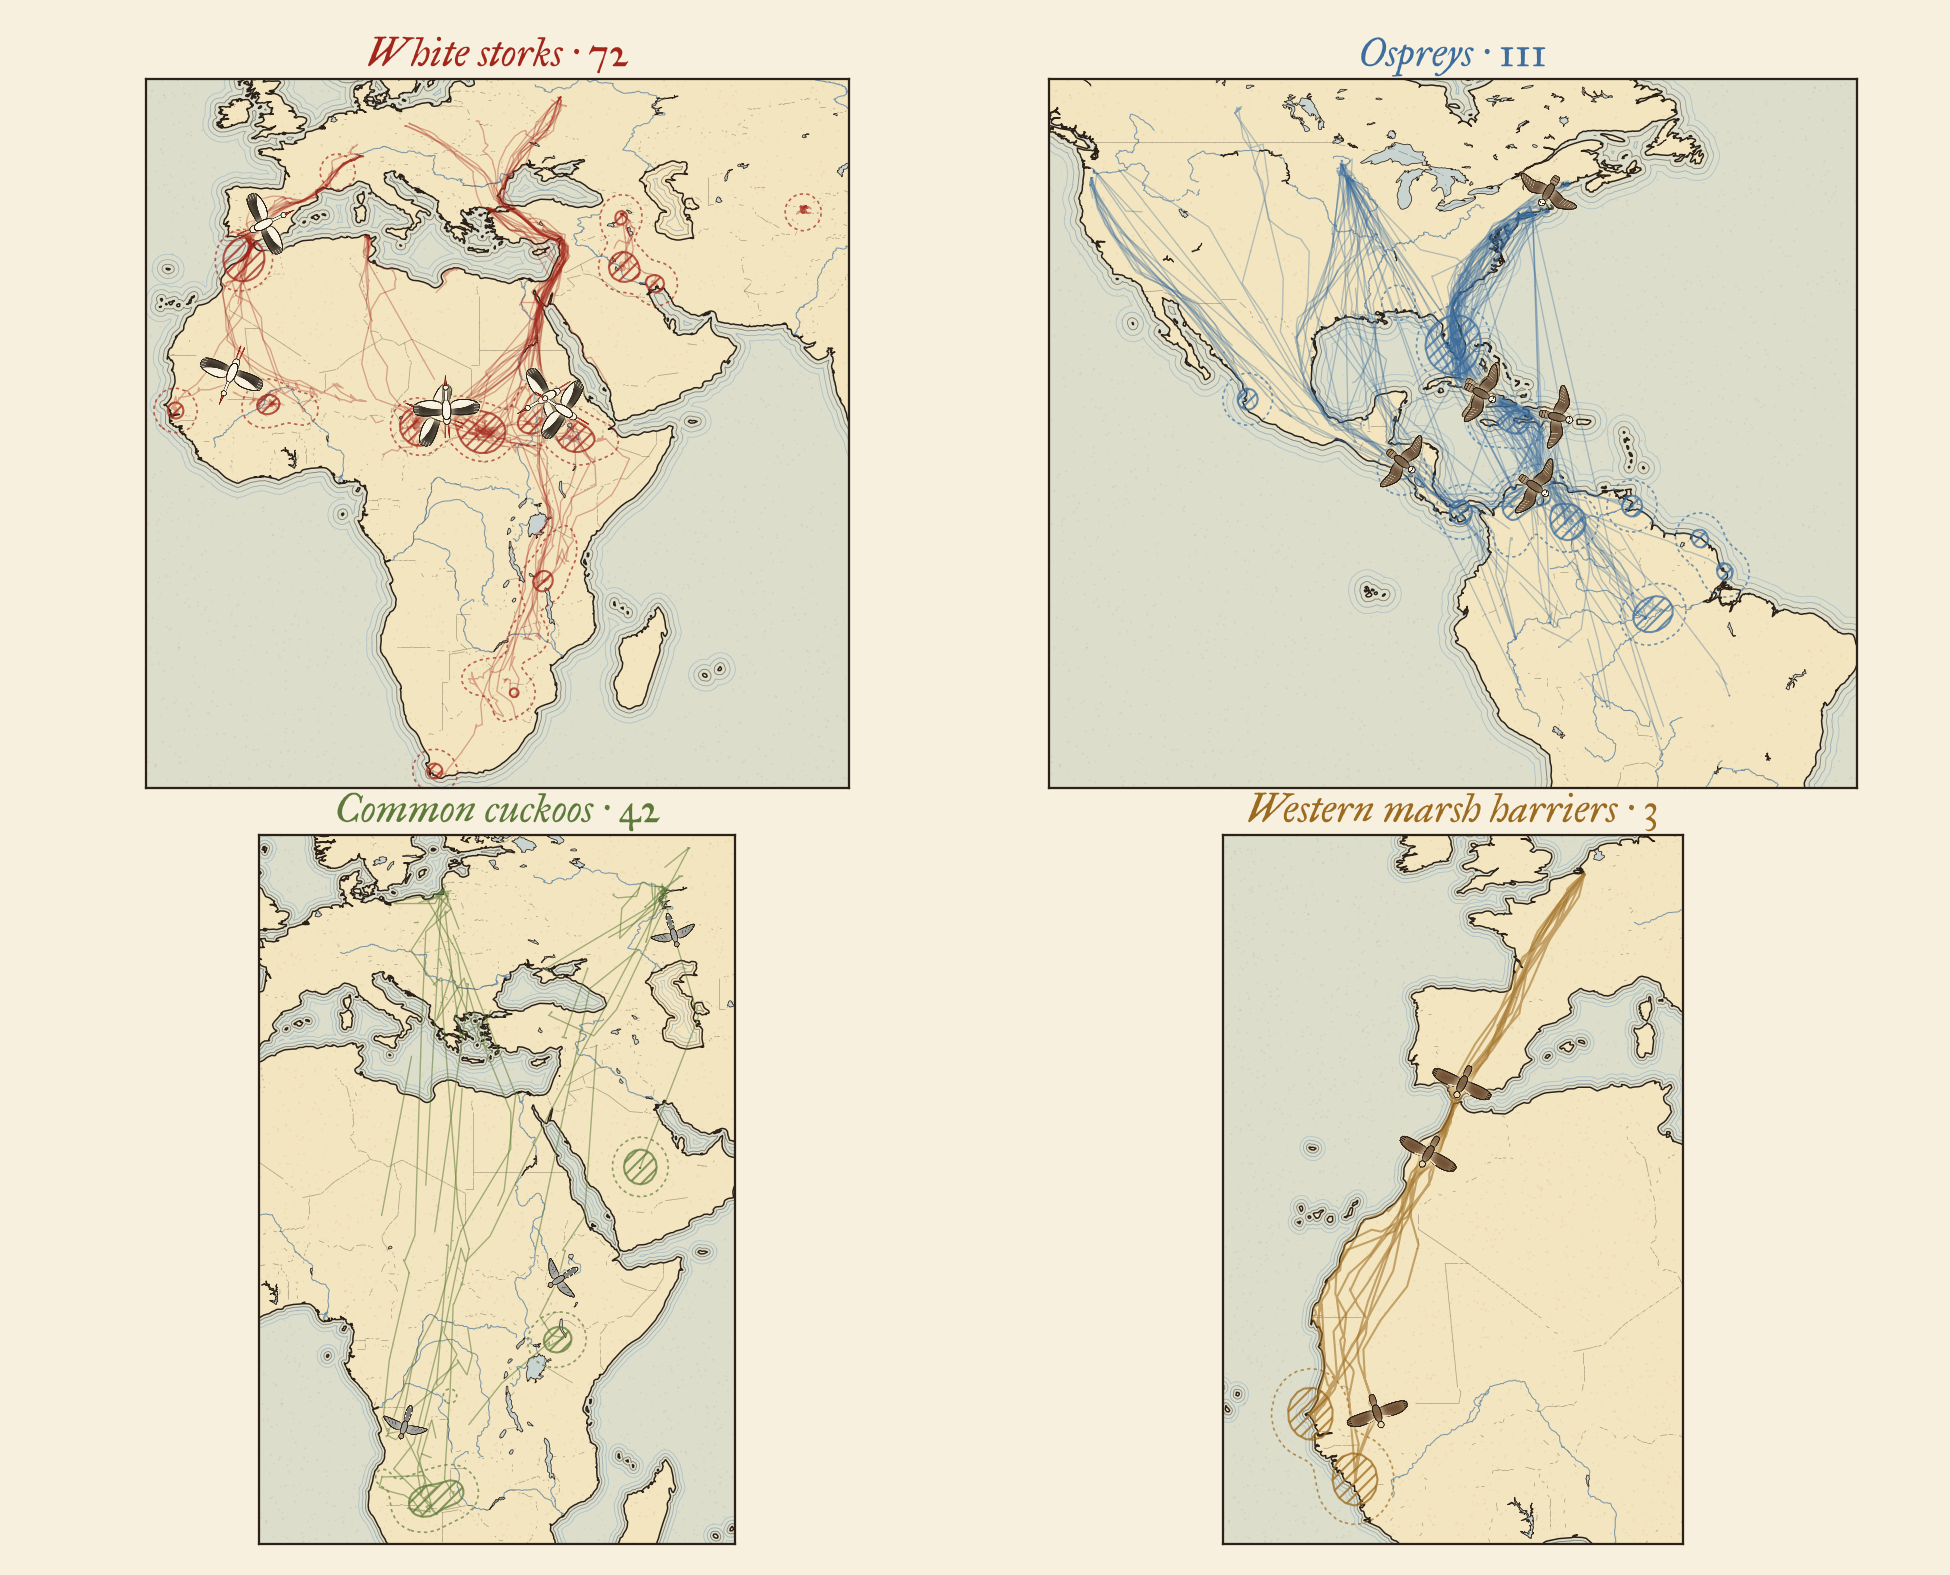
\includegraphics[width=\textwidth]{f_flyways.png}
\caption{Daily tracks of the four species (faint lines), with pen-drawn birds on sample autumn migrations and the winter quarters hatched (50\% of the December and January density; dashed: 90\%).}\label{fig:flyways}\end{figure}

\begin{figure}[tbp]\centering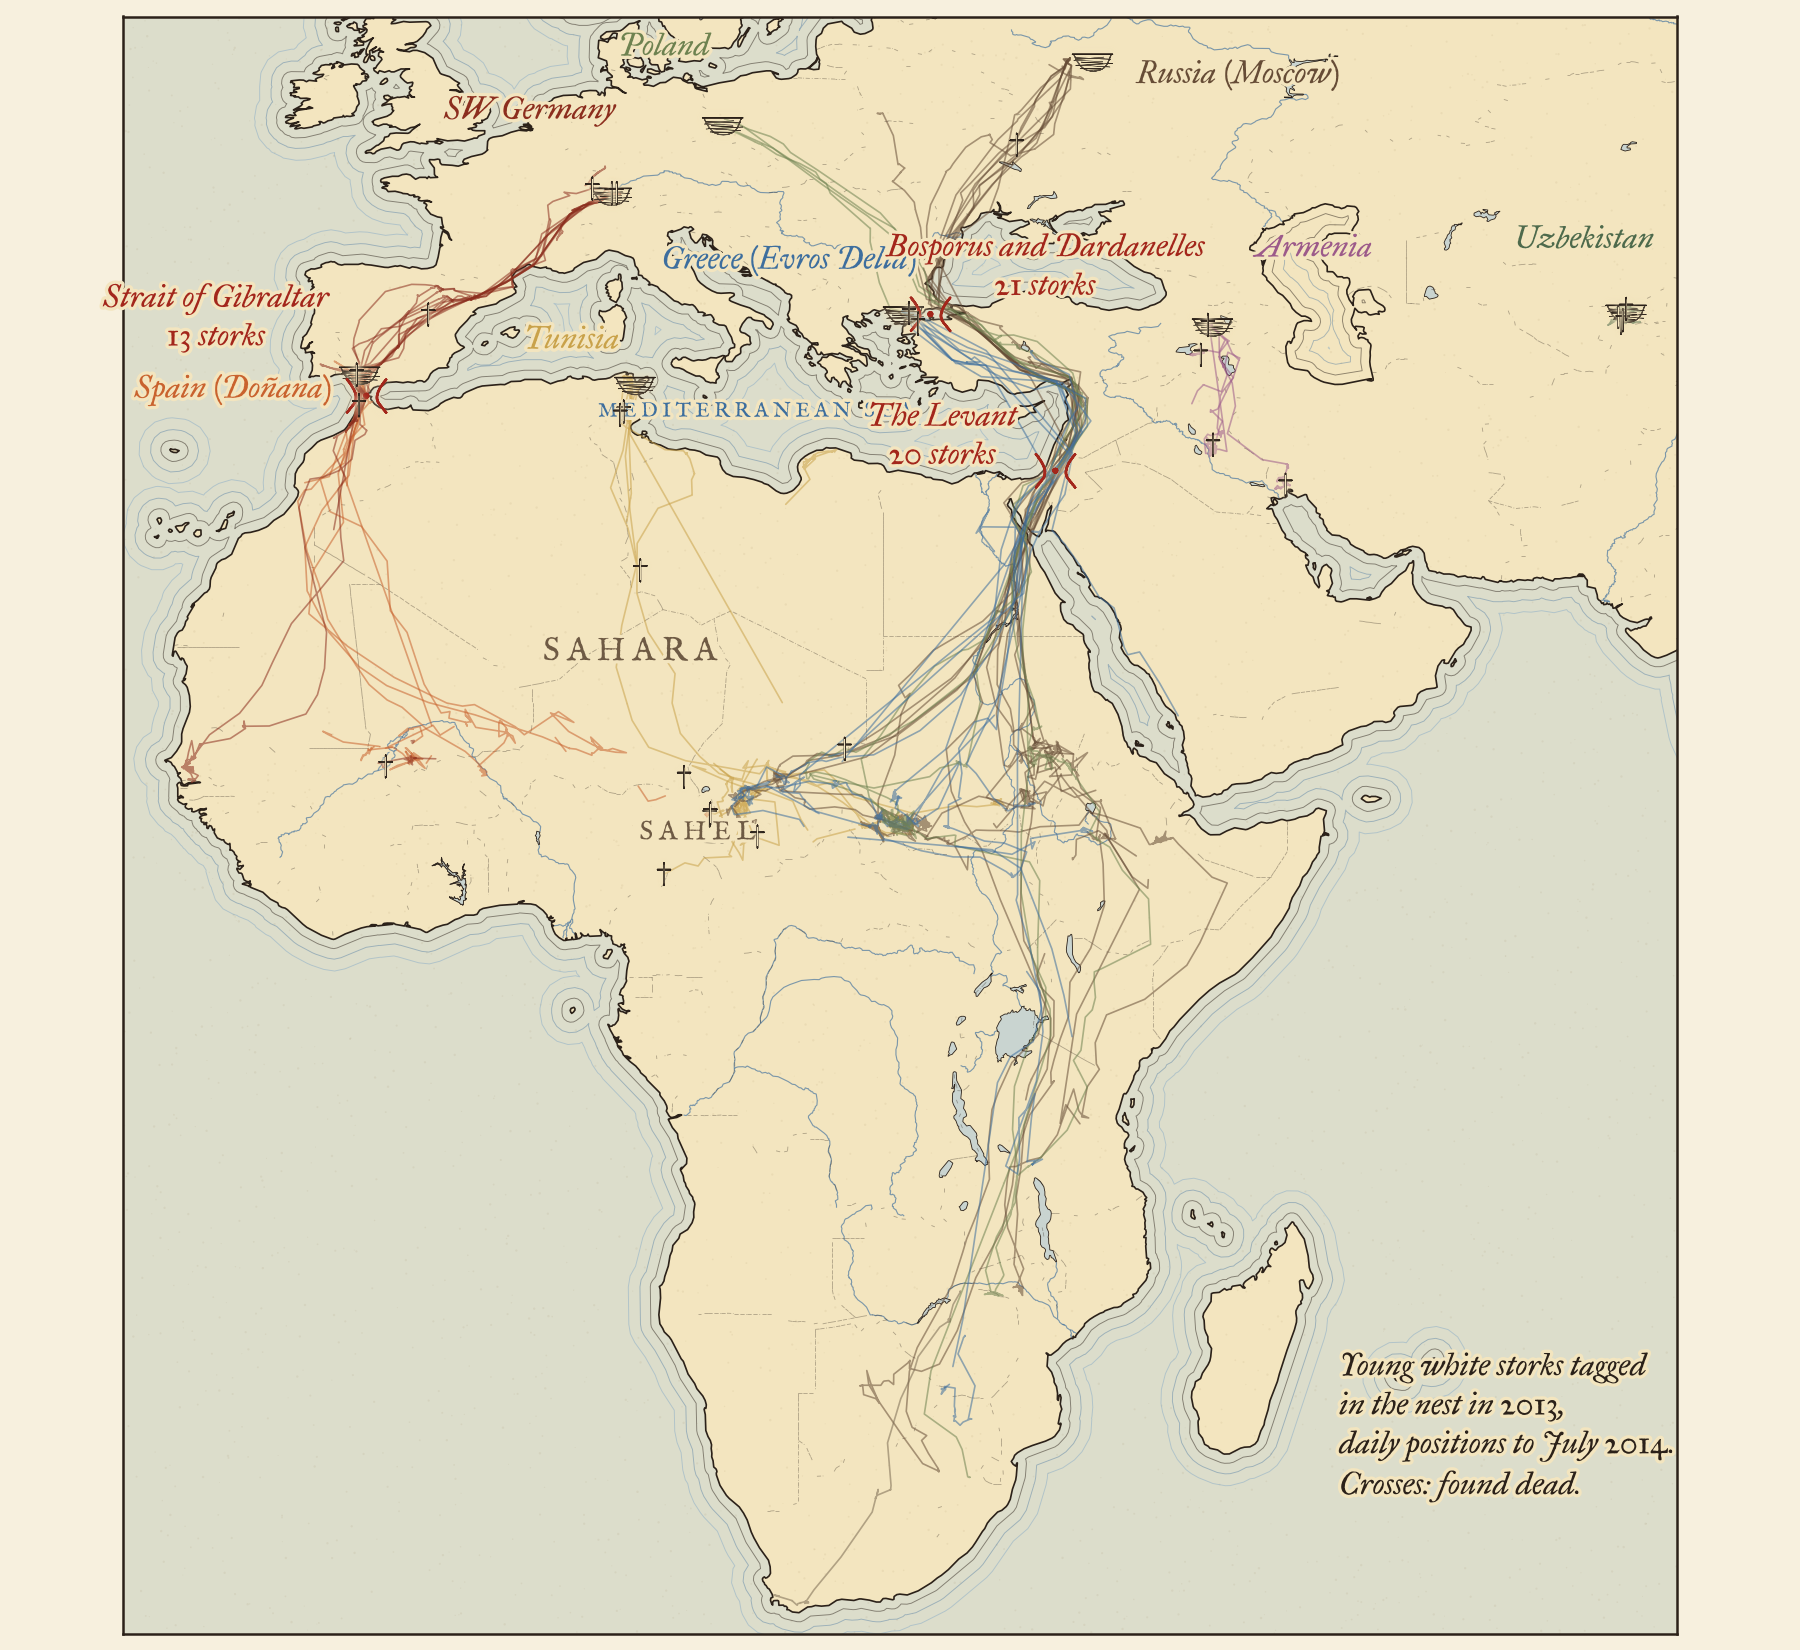
\includegraphics[width=0.92\textwidth]{f_storks.png}
\caption{Young white storks by population, with the three funnels and the last positions of birds found dead (crosses).}\label{fig:storks}\end{figure}

\subsection{Around the sea or across it}
Storks flew 0.61\% of their distance over the sea (2,360 of 389,086 km), and their longest run over water was 82 km (Figure~\ref{fig:sea}). Ospreys flew 22.0\% over the sea, about 36 times the storks' share; 4 made crossings of 300 km or more, mostly over the Caribbean between the Greater Antilles and northern South America (median 728 km). One osprey, KD, left Hispaniola, spent 82 hours over the Caribbean and returned to Haiti after 859 km. 4 cuckoos have straight lines between positions from southern Europe across the Mediterranean, the longest about 1,027 km; one young cuckoo went from Poland to Chad, 4,347 km, in 4.8 days. The harriers' longest crossing was 123 km.

\begin{figure}[tbp]\centering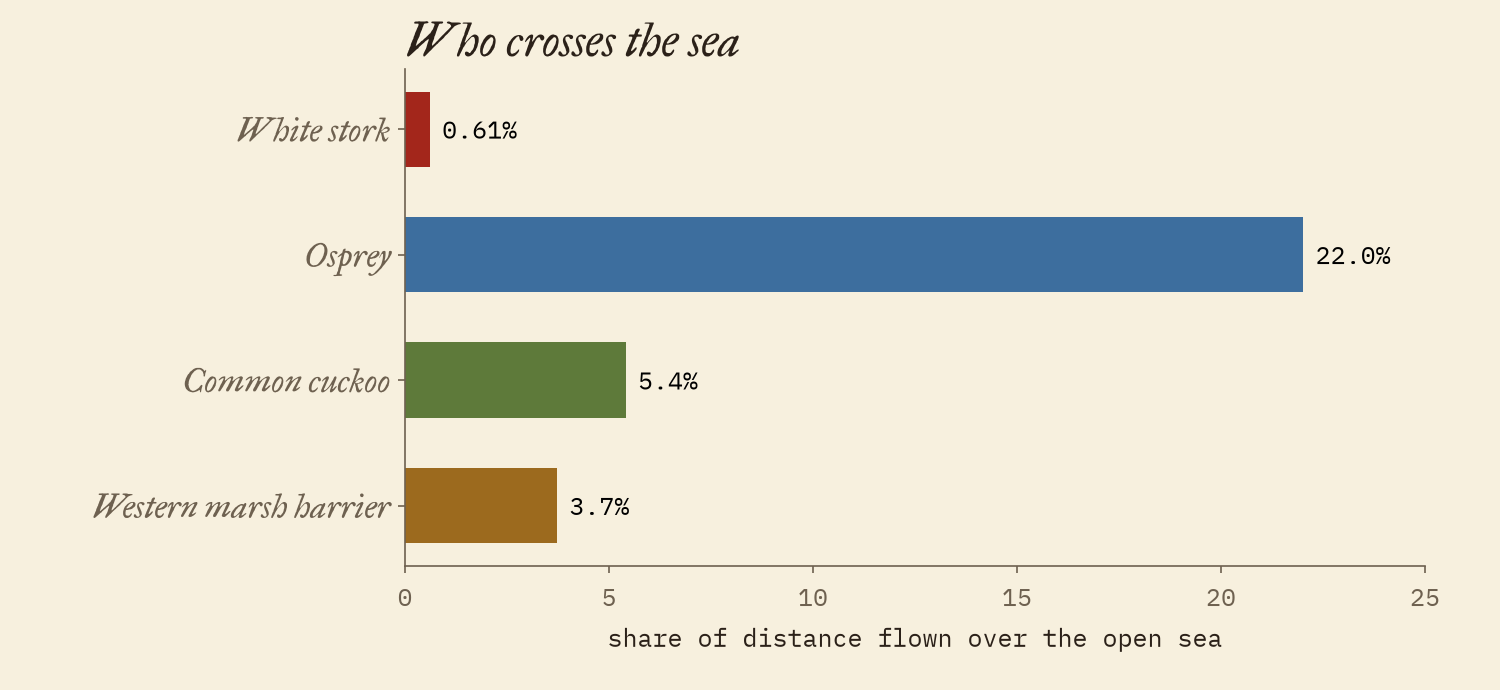
\includegraphics[width=0.85\textwidth]{f_sea.png}
\caption{Share of distance flown over the open sea, by species.}\label{fig:sea}\end{figure}

\subsection{Speed and distance}
\begin{table}[tbp]\centering\small\caption{Well-covered migrations: number, and medians of the distance between daily positions (km), the straight distance between anchors (km), days, km a day and days with more than 50 km of flight.}\label{tab:migr}\begin{tabular}{llrrrrrr}\toprule Species & Season & n & Path & Straight & Days & km/day & Travel days\\\midrule
White stork & autumn & 17 & 4,829 & 3,298 & 61 & 79 & 16\\
White stork & spring & 12 & 3,978 & 3,114 & 52 & 76 & 18\\
Osprey & autumn & 22 & 5,301 & 3,975 & 24 & 170 & 6\\
Osprey & spring & 8 & 4,977 & 3,786 & 23 & 237 & 3\\
Western marsh harrier & autumn & 5 & 4,639 & 4,492 & 51 & 89 & 19\\
Western marsh harrier & spring & 3 & 4,719 & 4,491 & 36 & 135 & 22\\
\bottomrule\end{tabular}\end{table}
Table~\ref{tab:migr} and Figure~\ref{fig:speed} summarise the well-covered migrations. Stork autumn migrations covered a median 4,829 km in 61 days, 79 km a day including stops, with a detour of 18\% over the straight line between anchors; ospreys went 2.1 times as fast. Cuckoo tracks were too sparse for this measure. The best day of the median migrating stork was 371 km and the best of all 558 km; ospreys reached 730 km and a marsh harrier 871 km, from central Spain to Morocco with flight continuing after dark. Over a year, 17 storks covered a median 12,724 km between daily positions and at most 23,680 km; between hourly positions the stork tracks are 41\% longer.

\begin{figure}[tbp]\centering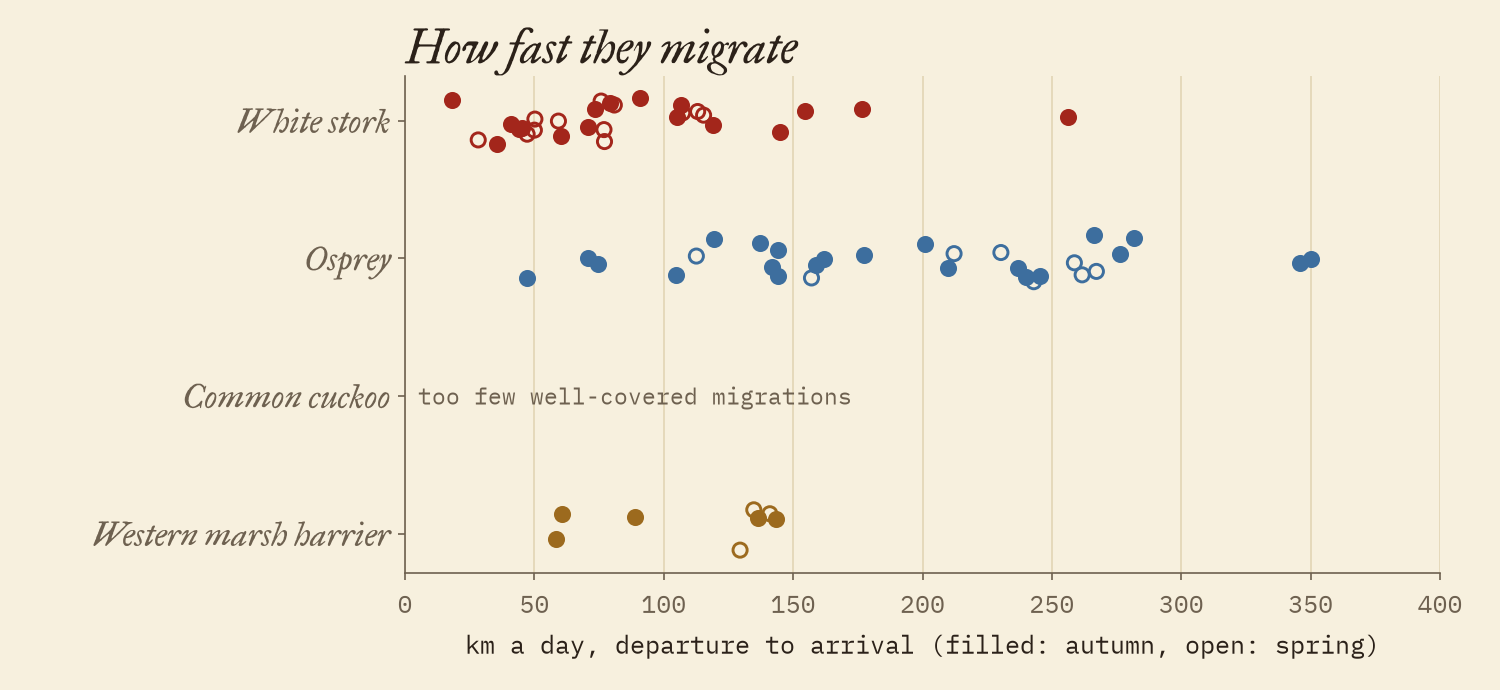
\includegraphics[width=0.85\textwidth]{f_speed.png}
\caption{Speed of each well-covered migration (distance between daily positions over days from departure to arrival).}\label{fig:speed}\end{figure}

\subsection{Winter quarters}
18 of the 34 storks with a winter position spent December and January in the Sahel belt (5 to 20°N), 5 in East and southern Africa and 5 in Europe and Morocco (Figure~\ref{fig:winter}). The farthest, DER AR445 from Moscow, reached Zimbabwe, 9,186 km from its nest. Of 65 ospreys tracked south of 25°N, 38 reached South America; 13 went no farther than Mexico, 9 of them from the western population. The two long-tracked harriers wintered at the same sites every year: Lilla's winter centres near Dakar in three winters lay within 2.6 km of each other, and Lillo's in Guinea 0.8 km apart (Figure~\ref{fig:harriers}).

\begin{figure}[tbp]\centering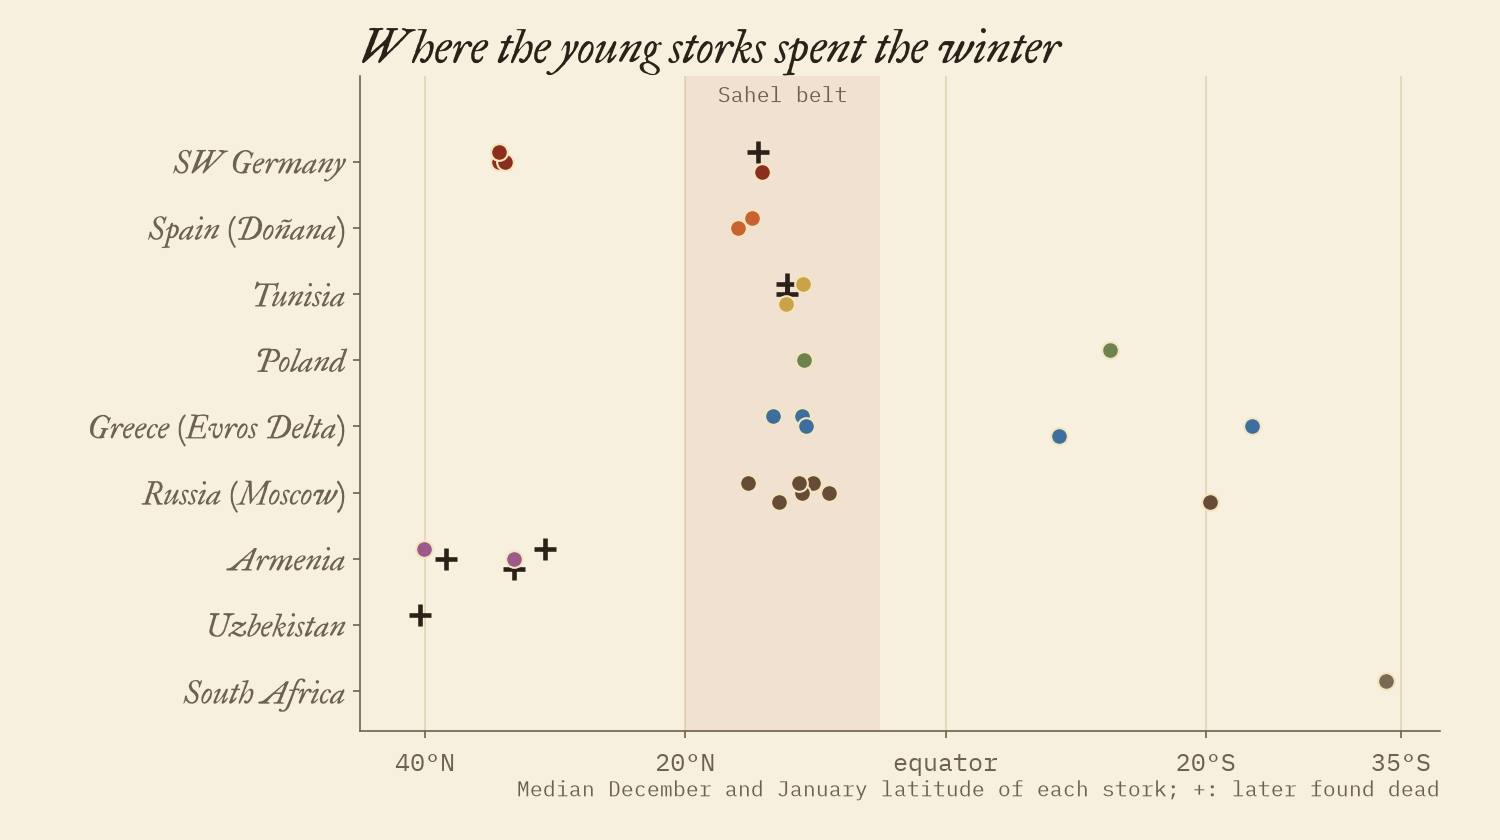
\includegraphics[width=0.85\textwidth]{f_winter.png}
\caption{Median December and January latitude of each stork, by population; crosses mark birds later found dead.}\label{fig:winter}\end{figure}

\begin{figure}[tbp]\centering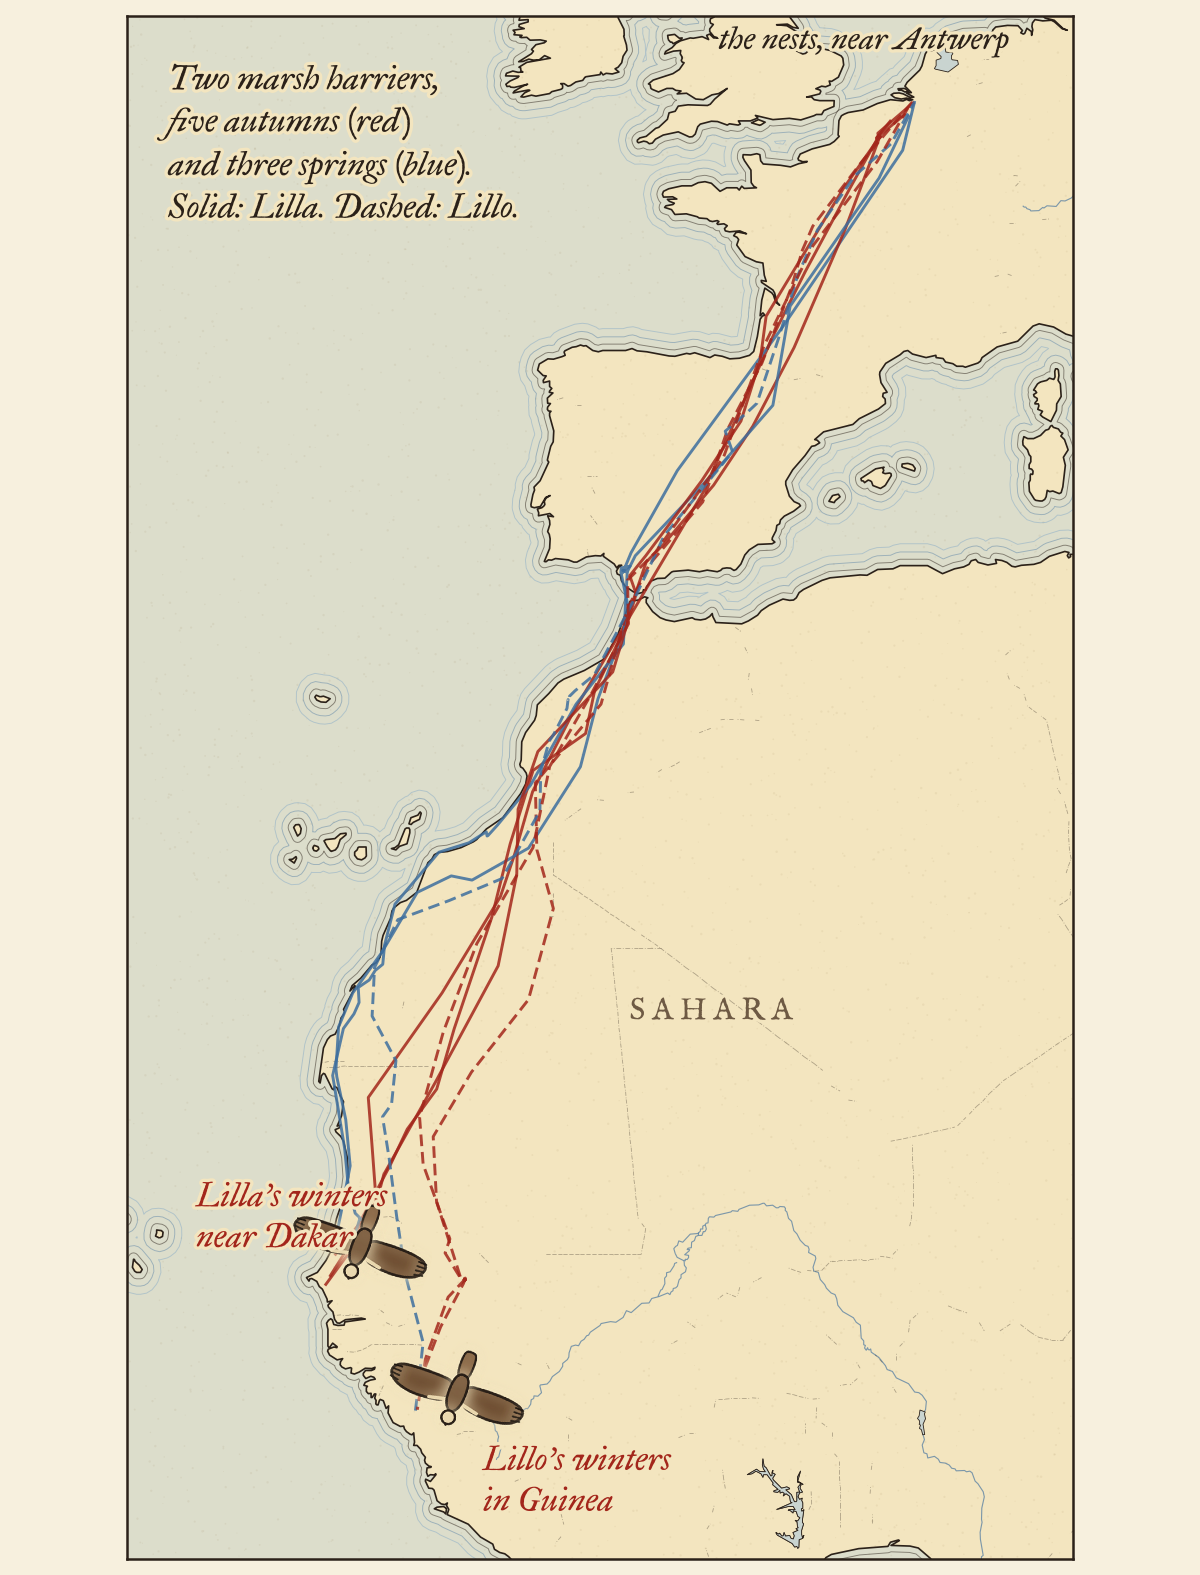
\includegraphics[width=0.62\textwidth]{f_harriers.png}
\caption{The migrations of two marsh harriers from Antwerp: autumn in red, spring in blue.}\label{fig:harriers}\end{figure}

\subsection{Fates}
30 of the 72 storks were confirmed dead (42\%); 16 of them never went 300 km from home and 15 died before 1 October 2013 (Figure~\ref{fig:fates}). Among birds that left home, deaths were 3 of 23 on the eastern route, 4 of 18 on the western route and 5 of 7 for Tunisian birds crossing the Sahara. These small numbers are descriptive only; \citet{flack2016} analyse the costs of the routes in detail. The osprey records note 8 deaths, 3 of them probably on floating debris at sea.

\begin{figure}[tbp]\centering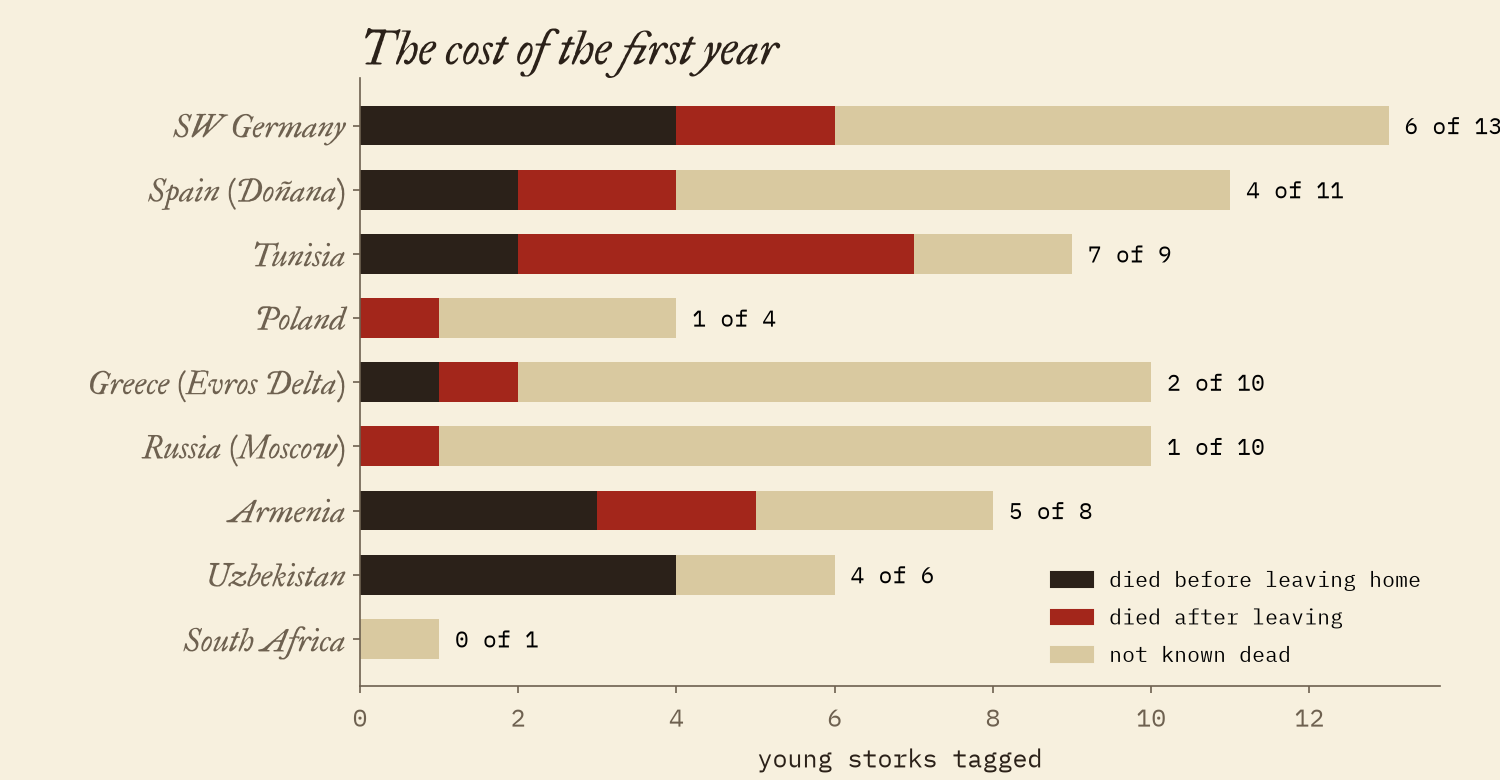
\includegraphics[width=0.85\textwidth]{f_fates.png}
\caption{Young storks by population: died before leaving home, died after leaving, and not known to have died.}\label{fig:fates}\end{figure}

\subsection{The displaced cuckoos}
Of the displaced cuckoos whose first 500 km from Kazan could be followed, 8 of 9 headed south-west (median bearing 201 degrees), against a median 176 degrees for 14 control birds (Figure~\ref{fig:cuckoos}). Tags were short-lived (median 53 and 26 days), so the end points are not known for most; \citet{thorup2020} give the full analysis.

\begin{figure}[tbp]\centering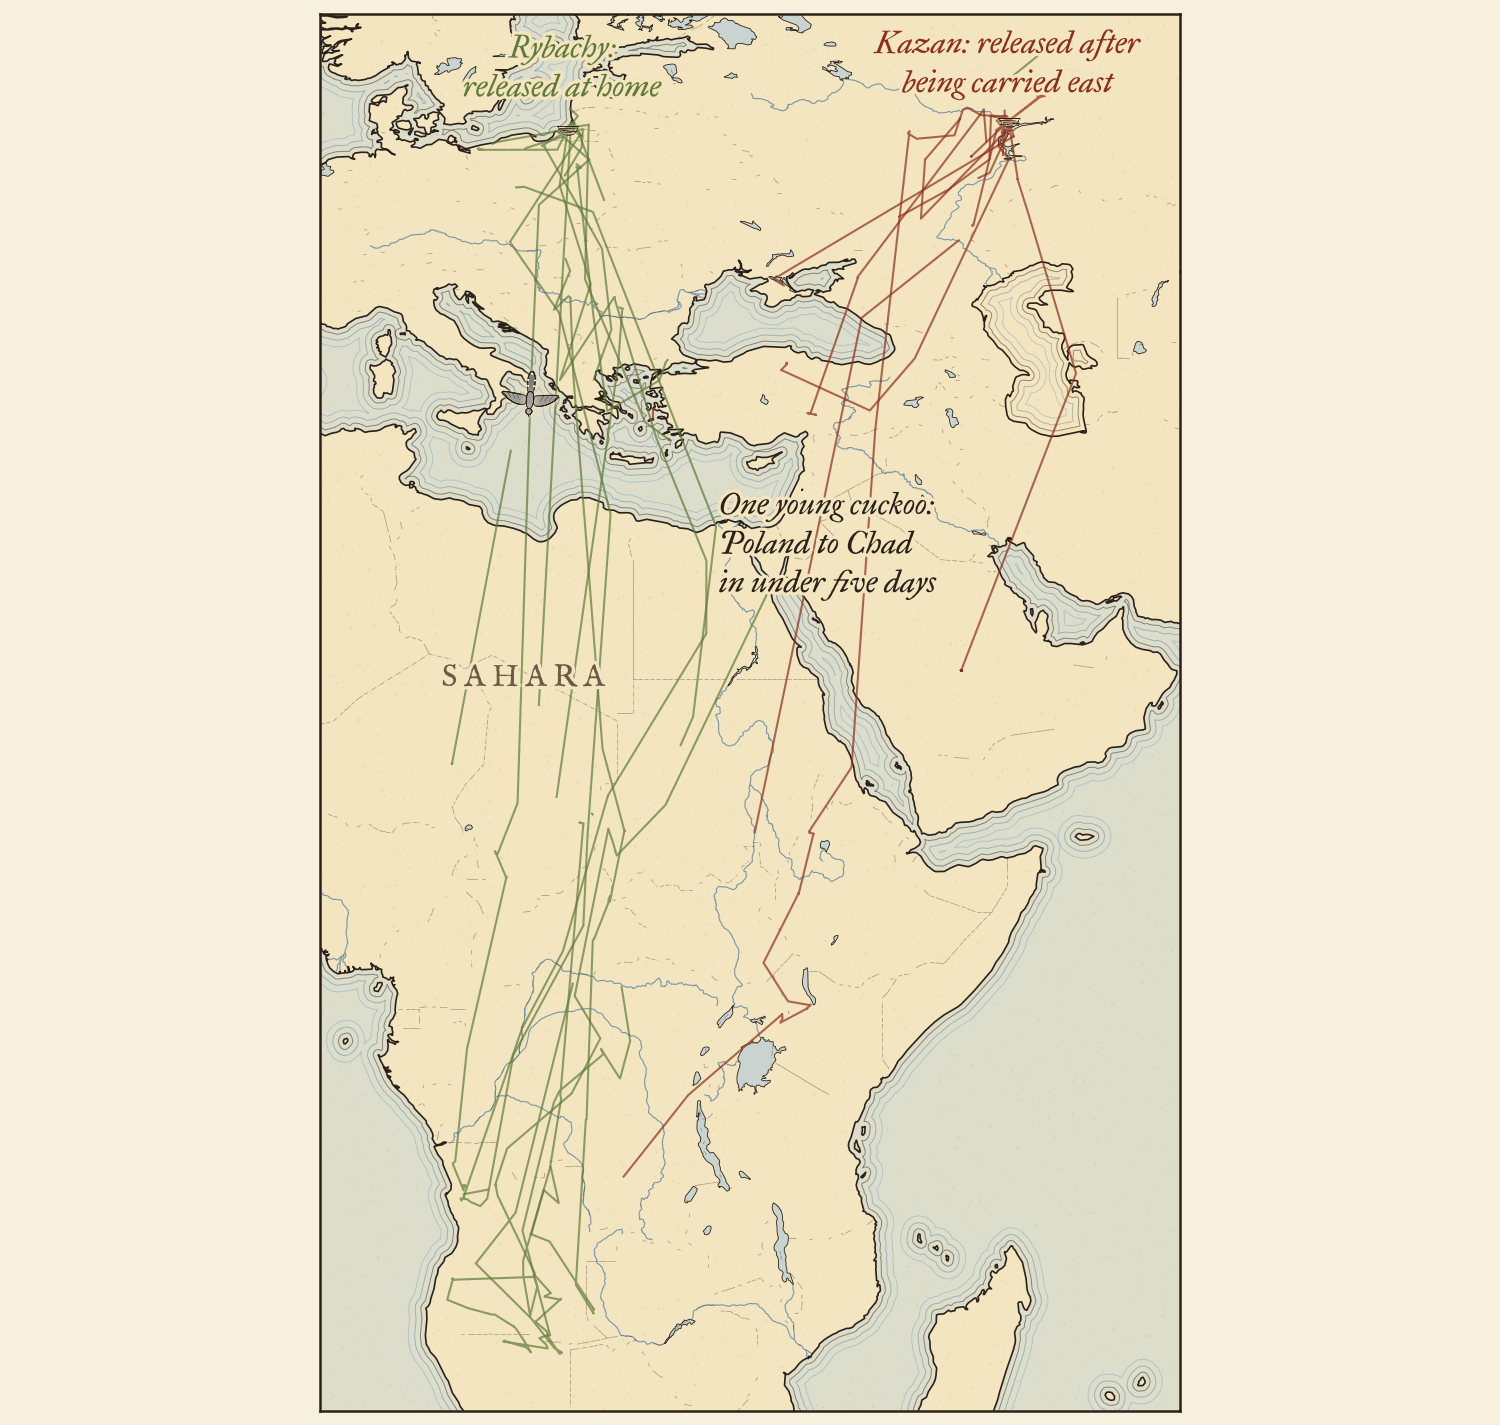
\includegraphics[width=0.75\textwidth]{f_cuckoos.png}
\caption{Cuckoos released at Rybachy (green) and after displacement to Kazan (red).}\label{fig:cuckoos}\end{figure}

\section{Limitations}
First, the samples are small and specific: one cohort of young storks in one year, ospreys of the late 1990s and three harriers; they describe these birds, not their populations. Second, satellite tags give a few positions a day with gaps of days, so osprey and cuckoo tracks are straight lines between sparse points; sea crossings and speeds are approximate for them and distances are lower bounds for all species. Third, the anchors and thresholds that define migrations, funnels and leaving home are choices; others would shift individual birds. Fourth, a tag that stops is not a dead bird: only deaths confirmed by the data owners are counted. Fifth, coastlines at 1:10m mislabel some positions on the shore as at sea. Finally, the cuckoo data come from an experiment, and the displaced birds' routes are not natural ones.

\section{Conclusion}
Put on one map, the four data sets show four ways of crossing the same barriers. The soaring storks treat the Mediterranean as a wall and squeeze through its narrowest gaps, and the young storks of Europe divide cleanly between Gibraltar and the Bosporus. Ospreys and cuckoos cross open sea, ospreys by day over the Caribbean and cuckoos by night over the Mediterranean and the Sahara. Harriers return year after year to the same few kilometres of West Africa. And the first year is costly: four young storks in ten did not survive it.

\section*{Data and code availability}
The interactive map is at \url{https://maps.tristanhotham.com/bird-migration/}. Data and code are at \url{https://github.com/Tristan-Hotham/bird-migration} and archived with this paper at https://doi.org/10.5281/zenodo.24043676. Derived data are released under CC BY 4.0 and code under the MIT licence; the tracking data are CC0.

\section*{AI statement}
I wrote the text, with drafting and editing assistance from Claude (Anthropic), which also helped prepare the analysis code. I reviewed and checked all text and results.

\begin{thebibliography}{12}
\bibitem[Douglas et al.(2012)]{douglas2012} Douglas, D. C., Weinzierl, R., Davidson, S. C., Kays, R., Wikelski, M. and Bohrer, G. (2012) Moderating Argos location errors in animal tracking data. \textit{Methods in Ecology and Evolution} 3: 999 to 1007. \url{https://doi.org/10.1111/j.2041-210X.2012.00245.x}
\bibitem[Flack et al.(2015)]{flackdata} Flack, A., Fiedler, W., Blas, J. et al. (2015) Data from: Migration costs of eight Eurasian white stork populations. Movebank Data Repository. CC0. \url{https://doi.org/10.5441/001/1.78152p3q}
\bibitem[Flack et al.(2016)]{flack2016} Flack, A., Fiedler, W., Blas, J. et al. (2016) Costs of migratory decisions: a comparison across eight white stork populations. \textit{Science Advances} 2: e1500931. \url{https://doi.org/10.1126/sciadv.1500931}
\bibitem[INBO(2023)]{inbo} Research Institute for Nature and Forest (INBO) (2023) MH\_ANTWERPEN: Western marsh harriers (\textit{Circus aeruginosus}, Accipitridae) breeding near Antwerp (Belgium). Zenodo, version 5. CC0. \url{https://doi.org/10.5281/zenodo.8238402}
\bibitem[Kays et al.(2015)]{kays2015} Kays, R., Crofoot, M. C., Jetz, W. and Wikelski, M. (2015) Terrestrial animal tracking as an eye on life and planet. \textit{Science} 348: aaa2478. \url{https://doi.org/10.1126/science.aaa2478}
\bibitem[Martell et al.(2001)]{martell2001} Martell, M. S., Henny, C. J., Nye, P. E. and Solensky, M. J. (2001) Fall migration routes, timing, and wintering sites of North American ospreys as determined by satellite telemetry. \textit{The Condor} 103: 715 to 724.
\bibitem[Martell and Douglas(2019)]{martelldata} Martell, M. S. and Douglas, D. (2019) Data from: Fall migration routes, timing, and wintering sites of North American ospreys as determined by satellite telemetry. Movebank Data Repository. CC0. \url{https://doi.org/10.5441/001/1.sv6335t3}
\bibitem[Natural Earth(2026)]{naturalearth} Natural Earth (2026) Admin 0 countries, lakes and populated places. Public domain. \url{https://www.naturalearthdata.com/}
\bibitem[Thorup et al.(2020a)]{thorupdata} Thorup, K., Vega, M. L., Snell, K. R. S. et al. (2020) Data from: Flying on their own wings: young and adult cuckoos respond similarly to long-distance displacement during migration. Movebank Data Repository. CC0. \url{https://doi.org/10.5441/001/1.vk36vq82}
\bibitem[Thorup et al.(2020b)]{thorup2020} Thorup, K., Vega, M. L., Snell, K. R. S. et al. (2020) Flying on their own wings: young and adult cuckoos respond similarly to long-distance displacement during migration. \textit{Scientific Reports}. \url{https://doi.org/10.1038/s41598-020-64230-x}
\end{thebibliography}

\clearpage
\appendix
\section{The young storks}
{\footnotesize\setlength{\tabcolsep}{4pt}\begin{longtable}{llllrrll}\caption{The 72 young storks: first and last daily position, distance between daily positions (km), farthest distance from the nest (km), winter country and confirmed deaths.}\label{tab:storks}\\\toprule Stork & Population & First & Last & km & Farthest & Winter & Fate\\\midrule\endfirsthead\toprule Stork & Population & First & Last & km & Farthest & Winter & Fate\\\midrule\endhead
BraveHeart (DER AP926) & Armenia & 2013-06-16 & 2014-01-22 & 2,290 & 1,134 & Iran & dead\\
DER AP921 & Armenia & 2013-06-16 & 2013-09-26 & 142 & 29 &  & dead\\
DER AP922 & Armenia & 2013-06-16 & 2013-12-13 & 960 & 236 & Turkey & dead\\
DER AP923 & Armenia & 2013-06-16 & 2013-11-25 & 952 & 535 &  & \\
DER AP924 & Armenia & 2013-06-16 & 2014-03-04 & 1,015 & 790 & Iraq & dead\\
DER AP925 & Armenia & 2013-06-17 & 2014-02-12 & 87 & 19 & Armenia & \\
DER AP927 & Armenia & 2013-06-16 & 2013-09-11 & 94 & 27 &  & dead\\
DER AP928 & Armenia & 2013-06-17 & 2014-06-15 & 3,854 & 866 & Iraq & \\
Dimitris (GRA51162) & Greece (Evros Delta) & 2013-07-03 & 2013-08-24 & 128 & 111 &  & dead\\
Hercules (GRA51167) & Greece (Evros Delta) & 2013-07-02 & 2013-09-02 & 638 & 513 &  & \\
Lina (GRA51160) & Greece (Evros Delta) & 2013-07-02 & 2013-09-14 & 3,672 & 2,852 &  & dead\\
Nenni (GRA51165) & Greece (Evros Delta) & 2013-07-02 & 2014-04-01 & 10,203 & 3,353 & Sudan & \\
Pelopidas (GRA51164) & Greece (Evros Delta) & 2013-07-02 & 2014-07-02 & 18,982 & 7,212 & South Africa & \\
Petros (GRA51163) & Greece (Evros Delta) & 2013-07-02 & 2014-04-15 & 8,605 & 5,623 & Tanzania & \\
Silvia (GRA51159) & Greece (Evros Delta) & 2013-07-02 & 2014-07-02 & 14,164 & 3,719 & Sudan & \\
Sophokles (GRA51157) & Greece (Evros Delta) & 2013-07-02 & 2013-10-28 & 4,448 & 3,290 &  & \\
Spithas (GRA51158) & Greece (Evros Delta) & 2013-07-02 & 2014-02-09 & 7,276 & 3,570 & Ethiopia & \\
Vasilia (GRA51161) & Greece (Evros Delta) & 2013-07-02 & 2013-08-22 & 3,509 & 3,048 &  & \\
PLG 5P305 & Poland & 2013-07-16 & 2013-11-28 & 12,283 & 8,884 &  & \\
PLG 5P307 & Poland & 2013-07-16 & 2013-11-07 & 1,646 & 1,501 &  & dead\\
PLG 5P311 & Poland & 2013-07-16 & 2014-07-16 & 18,840 & 7,763 & Zambia & \\
PLG 5P312 & Poland & 2013-07-16 & 2014-07-16 & 15,916 & 4,754 & Sudan & \\
DER AR436 & Russia (Moscow) & 2013-07-12 & 2013-11-06 & 7,052 & 5,135 &  & \\
DER AR437 & Russia (Moscow) & 2013-07-12 & 2013-09-09 & 633 & 638 &  & dead\\
DER AR438 & Russia (Moscow) & 2013-07-12 & 2014-06-19 & 9,778 & 5,381 & Ethiopia & \\
DER AR439 & Russia (Moscow) & 2013-07-12 & 2013-12-03 & 9,364 & 6,750 &  & \\
DER AR440 & Russia (Moscow) & 2013-07-12 & 2014-07-12 & 19,089 & 5,187 & Sudan & \\
DER AR441 & Russia (Moscow) & 2013-07-12 & 2014-01-30 & 12,247 & 6,896 & Sudan & \\
DER AR442 & Russia (Moscow) & 2013-07-12 & 2014-03-29 & 7,258 & 5,263 & Chad & \\
DER AR444 & Russia (Moscow) & 2013-07-12 & 2014-07-12 & 22,004 & 8,015 & Ethiopia & \\
DER AR445 & Russia (Moscow) & 2013-07-12 & 2014-07-12 & 23,680 & 9,186 & Zimbabwe & \\
DER AR446 & Russia (Moscow) & 2013-07-12 & 2014-07-12 & 12,724 & 4,610 & Sudan & \\
Benjamin (DER AN867) & SW Germany & 2013-07-15 & 2013-08-09 & 0 & 0 &  & dead\\
Cherry (DER AN859) & SW Germany & 2013-06-24 & 2013-09-02 & 1,348 & 1,166 &  & dead\\
Coco (DER AN862) & SW Germany & 2013-06-24 & 2014-01-25 & 5,540 & 3,918 & Mali & dead\\
Eamy (DER AL585) & SW Germany & 2013-06-24 & 2014-06-24 & 5,016 & 1,979 & Morocco & \\
Kakau (DER AN864) & SW Germany & 2013-06-24 & 2013-12-21 & 568 & 396 & France & \\
Karamell (DER AL582) & SW Germany & 2013-06-24 & 2014-06-24 & 5,767 & 1,983 & Morocco & \\
Keks (DER AN860) & SW Germany & 2013-06-25 & 2013-08-22 & 1,927 & 1,770 &  & \\
Pieps (DER AL586) & SW Germany & 2013-06-25 & 2013-08-23 & 146 & 97 &  & dead\\
Sierit (DER AN858) & SW Germany & 2013-06-24 & 2014-06-24 & 4,038 & 2,028 & Morocco & \\
Swag (DER AL583) & SW Germany & 2013-06-24 & 2013-07-02 & 0 & 0 &  & dead\\
Willi (DER AN863) & SW Germany & 2013-06-24 & 2013-08-08 & 112 & 23 &  & dead\\
Yolo (DER AN861) & SW Germany & 2013-06-24 & 2014-06-24 & 12,050 & 4,451 & Senegal & \\
Zozu (DER AL581) & SW Germany & 2013-06-24 & 2014-06-24 & 4,138 & 1,979 & Morocco & \\
ZAC 9A69901 & South Africa & 2012-11-30 & 2013-04-07 & 2,812 & 2,246 & South Africa & \\
C64W & Spain (Doñana) & 2013-06-11 & 2013-07-20 & 3 & 21 &  & dead\\
C666 & Spain (Doñana) & 2013-07-15 & 2013-11-04 & 8,312 & 2,916 &  & dead\\
C703 & Spain (Doñana) & 2013-06-11 & 2013-07-09 & 3 & 22 &  & dead\\
C708 & Spain (Doñana) & 2013-06-11 & 2014-04-25 & 4,512 & 3,536 &  & dead\\
C70V & Spain (Doñana) & 2013-06-11 & 2013-11-17 & 4,327 & 2,735 &  & \\
C711 & Spain (Doñana) & 2013-06-11 & 2014-03-07 & 5,399 & 2,594 & Mali & \\
C7VH & Spain (Doñana) & 2013-06-12 & 2013-11-03 & 3,153 & 2,514 &  & \\
C7W0 & Spain (Doñana) & 2013-06-12 & 2013-08-01 & 397 & 313 &  & \\
C7X7 & Spain (Doñana) & 2013-06-12 & 2014-06-11 & 8,906 & 2,714 & Mali & \\
C8WN & Spain (Doñana) & 2013-06-12 & 2013-07-24 & 488 & 465 &  & \\
CAMF & Spain (Doñana) & 2013-06-17 & 2013-07-25 & 746 & 741 &  & \\
DER AP801 & Tunisia & 2013-06-08 & 2013-07-30 & 271 & 202 &  & dead\\
DER AP802 & Tunisia & 2013-06-08 & 2013-11-03 & 2,792 & 2,574 &  & dead\\
DER AP803 & Tunisia & 2013-06-08 & 2014-04-04 & 7,849 & 3,193 & Chad & dead\\
DER AP804 & Tunisia & 2013-06-08 & 2014-02-16 & 5,521 & 2,862 & Chad & dead\\
DER AP805 & Tunisia & 2013-06-08 & 2013-12-04 & 4,026 & 3,165 &  & dead\\
DER AP806 & Tunisia & 2013-06-08 & 2013-08-20 & 335 & 228 &  & dead\\
DER AP807 & Tunisia & 2013-06-08 & 2013-11-02 & 1,340 & 1,221 &  & dead\\
DER AP808 & Tunisia & 2013-06-08 & 2014-06-08 & 11,058 & 3,501 & Sudan & \\
DER AP809 & Tunisia & 2013-06-08 & 2014-06-08 & 13,016 & 3,361 & Sudan & \\
Dilya & Uzbekistan & 2013-06-01 & 2014-06-01 & 1,059 & 90 &  & dead\\
Grigori & Uzbekistan & 2013-06-01 & 2014-02-10 & 729 & 64 &  & dead\\
Halim & Uzbekistan & 2013-06-01 & 2013-12-24 & 993 & 95 & Uzbekistan & dead\\
Mansur & Uzbekistan & 2013-06-01 & 2013-08-09 & 180 & 26 &  & dead\\
Sayyid & Uzbekistan & 2013-06-01 & 2014-06-01 & 1,068 & 63 &  & \\
Shahlo & Uzbekistan & 2013-06-01 & 2014-06-01 & 1,280 & 141 &  & \\
\bottomrule\end{longtable}}
\end{document}
